This section gives an overview of the key components of the solver. Figure \ref{fig_architec} gives an overview 
of the most basic classes and the classes they have pointers to (access to). 

\begin{figure}[!b]
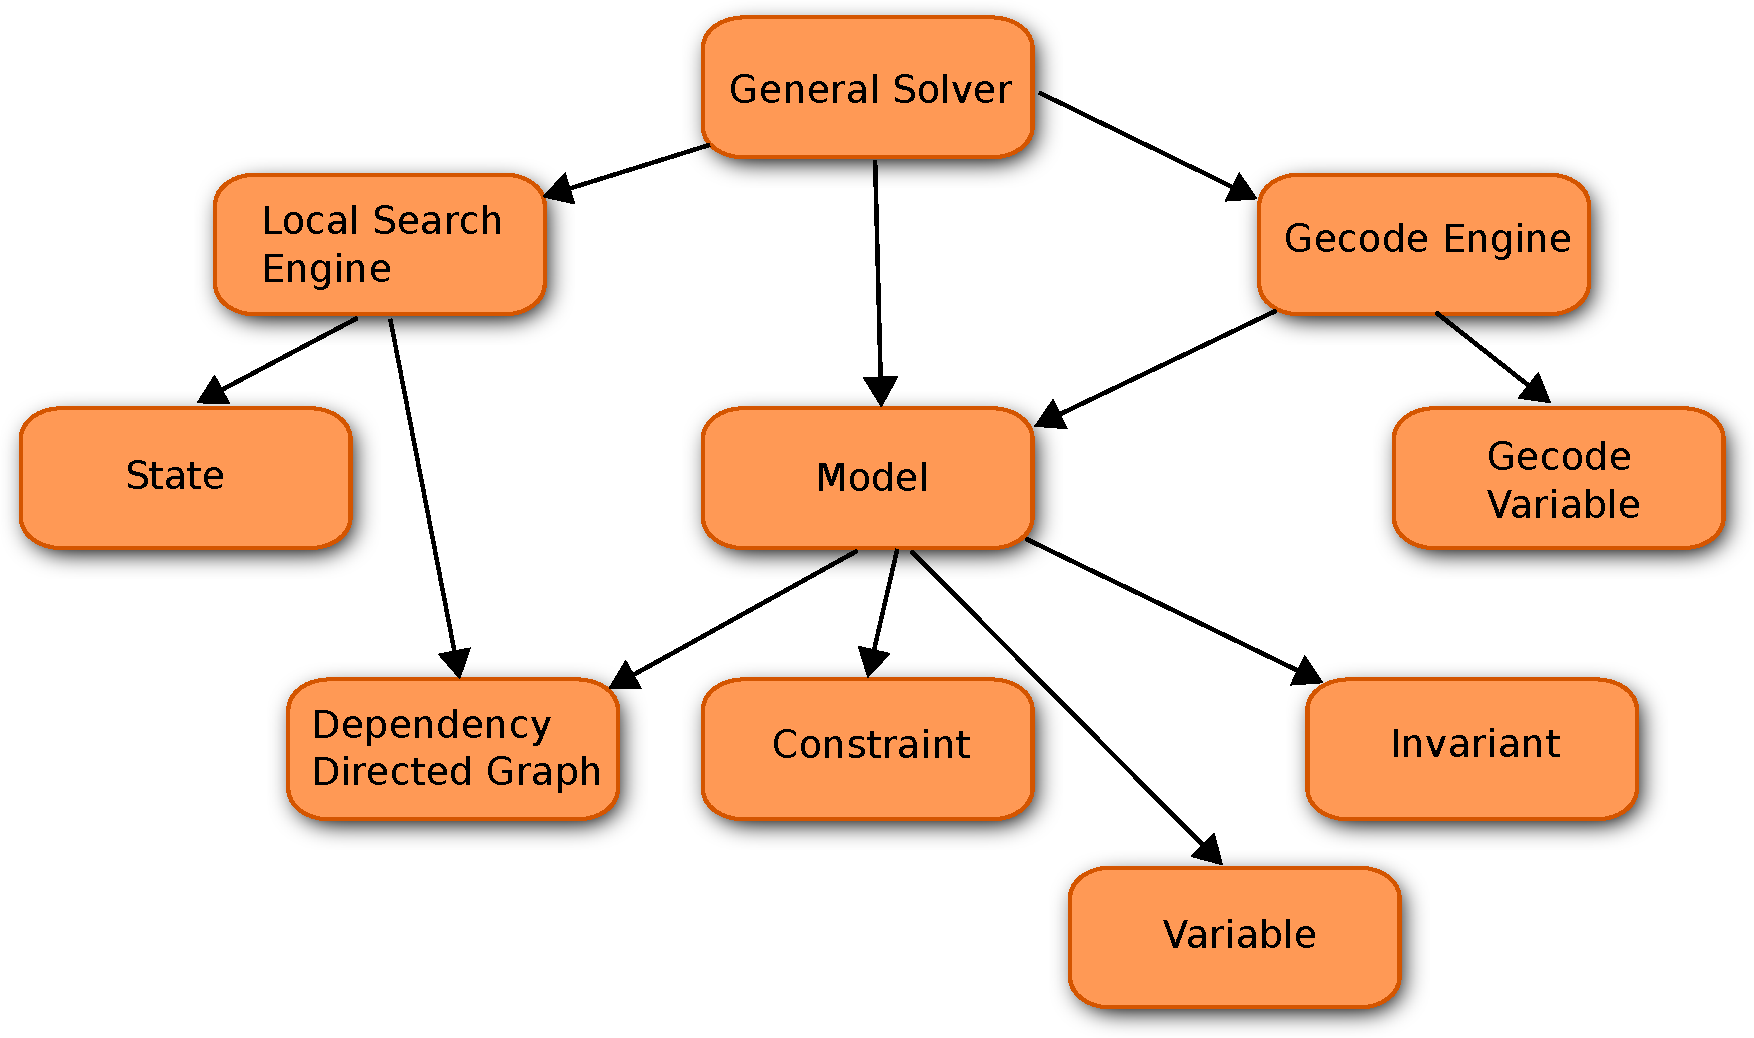
\includegraphics[width=\linewidth]{architectureTest}\caption{Overview of what the key classes of the framework contains 
pointers to} 
\label{fig_architec}
\end{figure} \noindent
The two engines for solving are the \gecodesol and \\ \lssol that find the initial solution and optimize the solution 
respectively. \gecodesol is used for preprocessing and finding an initial solution, if possible with in the limits 
given. \gecodesol will be elaborated further in section \ref{sec_gecode}. \\
\lssol is responsible for the optimization part of the solver with the use of local search and 
metaheuristics. How the optimization is done is described in section \ref{sec_local}. \lssol 
transform the model to a model better suited for local search before the local search can start. How this is done and 
why will be discussed in section \ref{sec_ls}. \\ 
The \class{Storage} class contains pointers to components of a CBLS model, variables, constraints, and invariants. 
\lssol can add new objects such as invariants to Storage. \\ 
\class{Constraint} and \class{Invariant} are super classes to all constraint and invariant respectively and are 
described in subsection \ref{sub_cons} and \ref{sub_inv}. They contain abstract methods that the subclasses must 
specify. \\ 
The main part of the solver is the \class{General Solver} class that contains the engines used for solving.
The \class{General Solver} class contains the methods that are called by the user, such as creating variables and 
constraints, finding initial solution and optimizing the solution and is described in subsection \ref{sub_gen}. \\ 
The \class{Variable} class contains both the variable used by Gecode but is also used for local search. 
